
\documentclass[conference]{IEEEtran}


\usepackage{cite}
\usepackage{listings}
\usepackage{amsmath}
\usepackage[tableposition=top]{caption}
\ifCLASSINFOpdf
\usepackage[pdftex]{graphicx}
\usepackage[pdftex]{color}
\usepackage{subcaption}
\else
\fi
\usepackage{url}
\usepackage{upquote}
\hyphenation{}


\begin{document}
\title{SpyREST: Automated Documentation for RESTful APIs using HTTP Proxy Server}


\author{\IEEEauthorblockN{S M Sohan, Craig Anslow, and Frank Maurer}
\IEEEauthorblockA{Department of Computer Science\\
University of Calgary\\
Calgary, Alberta T2N 1N4\\
Email: \{smsohan, craig.anslow, frank.maurer\}@ucalgary.ca  }
}
\maketitle


\begin{abstract}
Documentation of RESTful APIs are expensive to produce and maintain due to the lack of reusable tools and automated solutions for RESTful API documentation. Most RESTful APIs are documented manually and the API developers are responsible for keeping documentation up to date as the API evolves making the process both costly and error-prone. In this paper we introduce a novel technique using an HTTP proxy server that can be used to automatically generate RESTful API documentation and demonstrate SpyREST, an example implementation of the proposed technique. SpyREST uses a proxy to intercept example API calls and intelligently produces API documentation for RESTful Web APIs by processing the request and response data. Using the proposed HTTP proxy server based technique, RESTful API developers can significantly reduce the cost of producing and maintaining API documentation by replacing a large manual process with an automated process.
\end{abstract}

\IEEEpeerreviewmaketitle

\begin{IEEEkeywords}
RESTful API, Web API, Documentation, Automation, Example based documentation
\end{IEEEkeywords}


\section{Introduction}
RESTful APIs, introduced by Fielding, are used as a primary interconnection mechanism among modern day web based systems \cite{Fielding_rest}. For example, the website of a restaurant can use the RESTful API from Twitter to show the latest tweets mentioning the restaurant so that prospective customers can read the experience shared by others. To allow others to use their APIs, Twitter and other RESTful API developers publish documentation describing different features of their RESTful API. The documentation of such RESTful APIs are commonly produced and maintained using a manual process that is expensive.

API documentation for library APIs, such as Java Standard Edition, commonly leverage reusable tools such as JavaDoc. The documentation produced by such tools include description of objects and methods, with custom texts primarily sourced via comments in the source code. On the other hand, RESTful APIs documentation includes additional information such as HTTP headers, request parameters, request and response data in serialized formats such as JSON, XML, etc. that cannot be easily derived from looking at the objects and methods in the source code. Using comments for these additional information also requires significant manual effort because there is a lack of reusable tools to automate the documentation process. This makes the task of RESTful API documentation a costly and error-prone one. In addition to producing the API documentation, API developers also need to publish and often maintain the documentation for multiple versions as the RESTful API evolves. This requires further manual effort because it becomes a continuous process.

To produce RESTful API documentation with information about HTTP headers, URL parameters, request and response data, the manual process is driven by example API calls. This process can be described as a six-step process as follows: 1) craft an example call to an API endpoint with required headers, URL parameters and request body, 2) make the call, 3) capture the response headers and data, 4) strip any unwanted data from the captured information, 5) add custom descriptions to the captured data and 6) publish the API documentation. This six-step process is essentially repeated for all API endpoints that are documented. With \emph{SpyREST}, we have implemented an innovative solution to largely automate the aforementioned manual process of RESTful API documentation so that all but steps 1 and 5 are automated. Steps 1 and 5 are left to a manual process to allow for a pragmatic solution that leverages computers to automate the repeated part of the process while leaving the rest to humans. Our solution relies on a lightweight HTTP proxy server to intercept example API calls so that all the HTTP traffic for an API call can be automatically gathered. The collected data is then processed to present the documentation for RESTful APIs. Sensitive data such as authentication tokens and passwords are automatically filtered and are not captured. SpyREST can generate documentation for all RESTful APIs irrespective of the technology used to implement the API since it leverages an HTTP proxy server.

The key contributions of our research are as follows: we discuss a list of requirements for tool development to automate RESTful API documentation process and present a new technique based on an HTTP proxy server to meet the requirements. We demonstrate an example implementation of the proposed technique that generates automated yet customizable, version-aware, collaboration enabled and reusable API documentation software as a service platform that can be used to generate and maintain documentation for any RESTful API. We present a case study of using SpyREST to compare the advantages of our proposed technique over existing solutions for RESTful API documentation.

The remainder of this paper is organized as follows: in the next section we discuss the related work on API documentation. The implementation details of SpyREST is provided next. Then, we present a case study to demonstrate SpyREST in action. Then, we discuss the implications and limitations of our work in the discussion section.


\section{Related Work} % (fold)
\label{sec:related_work}
\subsection{General API Documentation} % (fold)
\label{ssub:api_learnability}
Several papers have studied the documentation of APIs to understand and recommend best practices that are also applicable to RESTful API documentation. Robillard et al. discussed the obstacles that make APIs hard to learn by surveying API developers and users \cite{Robillard_what_makes} \cite{Robillard_a_field_study}. They found that  developers faced severe obstacles learning new APIs due to inappropriate documentation and other learning resources. Robillard recommended the following for API documentation: include good examples, be complete, support many complex usage scenarios, be conveniently organized, and include relevant design elements. Kuhn et al. discussed the importance of examples in API documentation as a key recommendation based on a survey of software developers using APIs \cite{Kuhn_on_designing}. In addition to examples, they identified trustworthiness, confidentiality, and limiting information overload as other key recommendations for API documentation. Hoffman et al. recommended making the API example scenarios to be executable test cases so that a user can execute an API and understand the related business rules \cite{Hoffman_api_documentation}. We recognize all these recommendations to be equally important for RESTful APIs. SpyREST automatically generates RESTful API documents from example API calls, with information about the publisher and allows the users to execute the examples following the aforementioned recommendations.

Nasehi et al. performed a case study based on StackOverflow discussions to find out what makes good code examples \cite{Nasehi_what_makes}. They recommended API developers to include a comprehensive set of code examples in the API documentation and the use of wiki-like collaborative tools with online API documentation so that users can ask questions and get answers on officially published API documentation. Parnin et al. found that social media holds a key place in software documentation as  it provides additional knowledge about APIs and gives readers a chance to engage with authors of the APIs \cite{Parnin_measuring}. They found active collaboration about API related questions resulted into 81\% of posts receiving at least one comment with a median of 8 comments per question. Chen et al. recommended integrating crowdsourced frequently asked questions (FAQs) into API documents so that users can easily find relevant discussions when questions arise as they are browsing API documentation \cite{Chen_who_asked}. They presented a tool that can embed FAQs into API documents based on a user's browsing behavior. Subramanian et al. presented an automated approach to link API documentation of different Java and JavaScript libraries with code examples that are shared on StackOverflow by the API users so that the collaborative crowd documentation of APIs can be linked with official documentations \cite{Subramanian_live}. To link API documentation with valuable crowdsourced content, the collaborative features of SpyREST allows users to discuss API related questions and answers on the same web pages where the auto generated RESTful API documentations are shown.

Stepalina discussed the advantages of software as a service (SaaS) based solutions for API documentation systems where a web platform can be used to publish many different API documentations \cite{Stepalina_saas}. They identified several benefits of a SaaS platform, such as, cost effective yet powerful, platform agnostic and high accessibility, improved document quality, content re-use, automated tools, and organization of robust and scalable documentation process. SpyREST is a SaaS based tool that can be used to leverage these benefits as it allows the generation and publishing of RESTful API documentations for many different APIs under a single platform. They also identified security and reliability of such a shared platform as potentially open issues. To overcome these issues, SpyREST allows a self-hosted alternative to the SaaS model where a SaaS platform is not acceptable for RESTful API documentation.

Several tools exist that help automatic generation of API documentation for local APIs such as JavaDoc\footnote{http://www.oracle.com/technetwork/java/javase/documentation/index-jsp-135444.html}, RDoc\footnote{http://rdoc.sourceforge.net/}, that convert formatted comments from source code into corresponding HTML documentation for the classes and methods. Jadeite is a tool that adds placeholder API objects for library APIs to improve the search and discovery of desired API objects \cite{Jadeite}. While these tools have been proven to work for local library APIs, they have limited applicability for documenting RESTful APIs because HTTP specific information such as request and response headers, URL, request and response payloads are not natively supported by these tools. Hence, there exists a gap for tool support to automatically generate RESTful API documentation. SpyREST fills this gap as by automatically generating RESTful API documentation from example API calls.

\subsection{RESTful API Documentation} % (fold)
\label{sub:restful_api_documentation}

To address the need for a standard format to describe RESTful APIs, several related work proposed candidate specifications. Maleshkova et al. analyzed multiple Web APIs to identify the different approaches related to Web API descriptions, data formats, protocols, reusability, granularity, and authentication \cite{Maleshkova_investigating}. They found that a lack of a standard format to document Web APIs and manual documentation led to API under-specification causing confusions about how to use the APIs for different use cases. They identified a need for automated approaches. Espinha et al. observed that most RESTful APIs are documented manually by API developers making the documentation a less reliable one \cite{Espinha_web}. To standardize the terminology for RESTful API documentation, Danielsen et al. presented a vocabulary for documenting RESTful Web APIs called Web Interface Language (WIfL) \cite{Danielsen_validation}. The vocabulary comprises of these following objects: Resource, Request, Response, Representation and Parameters that can describe the structure and example usage of RESTful Web APIs. Generation of WIfL specific objects for RESTful APIs requires manual effort or bespoke implementation since a reusable automated approach is not presented. With SpyREST, we focus on automation so that reusable tools can be used to produce RESTful API documentation.

Verborgh et at. presented RESTdesc, a Resource oriented and Hyper-link based specification for describing RESTful APIs \cite{Verborgh_functional}. RESTdesc relies on pre and postconditions to describe the outcome of an API call so that a general purpose API client can parse RESTdesc formatted documentation to invoke API calls to specific RESTful APIs. Mangler et al. presented RDDL, an XML based specification for describing RESTful APIs \cite{Mangler_rddl}. RDDL descriptions are composed of resources, operations, parameters, and headers. Similar to WIfl, manual effort is needed to generate RESTdesc and RDDL formatted documentations.

Kopecky´ et al. presented hRESTS, a machine readable micro-format to describe RESTful APIs that use an alternate representation compared to WIfL \cite{Kopecky_hrests}. hRESTS specification comprises of Service, Operation, Address, Method, Input, Output and Label objects to describe RESTful APIs. Automated XML transformation is used to convert a formatted HTML documentation of a RESTful API into hRESTS so that the machine readable format can be used by RESTful API clients for automated invocation. Ning et al. presented OmniVoke, a RESTful API based invocation engine that provides an abstraction layer for RESTful API calls to multiple APIs that follow different conventions \cite{Ning_omnivoke}. A general purpose RESTful API client can be used against OmniVoke since the different conventions are wrapped under a uniform RESTful API. Manual configuration is required for each existing API to wrap under OmniVoke. SpyREST relies on example API calls and does not require APIs to be described according to a specification format. Instead, the data recorded by SpyREST can be used to automatically produce API descriptions following a specification as an output that otherwise requires manual effort.

Myers et al. performed a user study based on the documentation of Web APIs used in large scale enterprises to understand the required contents for Web API documentation \cite{Myers_study}. They recommended providing a consistent look-and-feel with explanation for the starting points and an overall map comprising of both text and diagrams, providing a browsing experience with breadcrumb trail following a hierarchy, an effective search interface, providing example code and a way to exercise the examples online without writing code. SpyREST aims to achieve requirements for RESTful API documentation using an automated yet customizable approach that can be reused across different RESTful APIs.

In addition to the research community, there are several RESTful API specification formats that are observed in the industry. Swagger is a JSON based specification that allows users to describe RESTful APIs in terms of paths, parameters, request and response headers and bodies\footnote{https://github.com/swagger-api/swagger-spec/blob/master/versions/2.0.md}. RAML is a RESTful API documentation format that uses YAML files to describe RESTful API documentation using a similar hierarchy as Swagger\footnote{http://raml.org/spec.html}. Blueprint is another RESTful API specification format that uses Markdown files with additional tags to describe RESTful API objects\footnote{https://github.com/apiaryio/api-blueprint}. In addition to producing RESTful API documentation, there are tools and software as a service (SaaS) providers that can be used to publish the documentation and auto generate API client code for RESTful APIs that are described using one of these formats. To use these tools to generate HTML based RESTful API documentation, API developers need to manually construct the intermediate documentation format such as Swagger, Blueprint, RAML, etc. that is required by these platforms since there is no automated tool to produce this. In contrast, SpyREST generates RESTful API documentation by synthesizing data collected from example API calls without relying on any intermediate representation.
% subsubsection restful_api_specification (end)


\section{SpyREST} % (fold)
\label{sec:spyrest}

\subsection{SpyREST Requirements} % (fold)
\label{sub:spyrest_requirements}

The following list of requirements for SpyREST, R1-7 in priority order, is derived from analyzing the aforementioned related work and current API documentation practices as observed in the industry:

  \textbf{R1 - Automated RESTful API documentation}: RESTful APIs are either documented manually or using custom tools to partially automate the process. Both processes can be expensive to maintain since API documentation is a continuous process to support the evolution of APIs. The primary requirement for SpyREST is to find a pragmatic approach to automate RESTful API documentation.

  \textbf{R2 - Example based}: As discussed in the related work section, several authors have emphasized on including example scenarios with API documentation can help users understand how to use an API \cite{Robillard_what_makes} \cite{Kuhn_on_designing} \cite{Hoffman_api_documentation} \cite{Nasehi_what_makes}. SpyREST generated API documentation needs to include example scenarios.

  \textbf{R3 - Executable documentation}: In addition to including examples, SpyREST also needs to allow users to execute the example scenarios so that they can try the API features without having to write code \cite{Hoffman_api_documentation} \cite{Myers_study}.

  \textbf{R4 - Version awareness}: SpyREST needs to allow API developers to publish documentation for multiple versions of a Web API as it evolves. The following comment from an API user of Stripe, an online payment processing company, shows the importance of a version-aware documentation tool\footnote{\url{https://groups.google.com/a/lists.stripe.com/forum/#!searchin/api-discuss/version/api-discuss/li4PyVcweiw/NT9SFTtF-vQJ}}
:
  \small
  \begin{quotation}
   ``Does the full API documentation only reflect the current version of the
    API?  Is there a way to access the API docs for outdated versions? ...That would be very helpful. When you are trying to upgrade from one version to another it's impossible to know the implementation differences. We are currently about 4 API versions behind and are stuck behind a version that causes a significant amount of work on our end to support. I'd like to be able to upgrade incrementally through each version.''
  \end{quotation}
  \normalsize

  \textbf{R5 - Customizable}: Robillard identified the importance of customized overview information about how to use an API to reduce API learning obstacles \cite{Robillard_what_makes}. Custom content is also required to explain business rules and overview information about APIs that may not be automatically derivable. SpyREST needs to allow users to add customized content to auto generated RESTful API documentation so that API developers can provide required information about the APIs that are not automatically generated.

  \textbf{R6 - Reusable}: SpyREST needs to work as a reusable platform so that multiple REST API documentations can be generated and published on a single platform to get the advantages of a SaaS platform as outlined by Stepalina \cite{Stepalina_saas}.

  \textbf{R7 - Collaborative}: SpyREST needs to allow people to collaborate on the API documentation so that questions and answers about APIs can coexist with the API documentation to overcome the obstacles with fragmented knowledge sources \cite{Chen_who_asked}.


\subsection{SpyREST Components} % (fold)
From our research to meet the requirements R1-7, we have identified an HTTP proxy server based solution as a novel approach for generating RESTful API documentation. A possible implementation and the related advantages of the HTTP proxy server based approach is demonstrated through SpyREST. SpyREST is composed of three main components as shown in Fig. \ref{fig:components}.

\begin{figure}[htb]
\centering
\def\svgwidth{\linewidth}
\input{components.pdf_tex}
\caption{SpyREST Component Diagram}
\label{fig:components}
\end{figure}

\textbf{The Spy:} SpyREST is driven by example calls to the RESTful APIs to generate the documentation for the APIs. The Spy component in SpyREST is an HTTP proxy server. The Spy is named so because it records the HTTP traffic for example API calls that are made using it as a proxy server. For example, when using Spy as an HTTP proxy to make the following HTTP request:

\footnotesize
\begin{description}
  \item[Method] GET
  \item[URL] https://api.github.com/repositories?since=100
  \item[Headers] accept: application/vnd.github.v3+json
\end{description}
\normalsize
that produces the following response:
\footnotesize
\begin{description}
  \item[Headers] status: 200 OK \\
content-type: application/json; charset=utf-8 \\
...
  \item[Body]
\begin{lstlisting}

[
  {
    "id": 1,
    "name": "grit",
    "full_name": "mojombo/grit",
    ...
  }
]\end{lstlisting}
\end{description}
\normalsize
Spy automatically saves the raw request and response data with HTTP headers. Additionally, the Spy synthesizes the data and saves the following meta data about this example API call:

\footnotesize
\begin{tabular}{r p{0.55\linewidth}}
  version & v3 \\
  resource & repositories \\
  action & GET /repositories \\
  query & since: 100 \\
  strippedResponseBody & a subset of the response body \\
  description & blank \\
  digest & base64 hash value of the version, resource, url and description \\
  requiresAuth & false \\
  apiToken & blank, used when a SpyREST API token is provided \\
  userId & blank, used when a user is found for given apiToken \\
\end{tabular}
\normalsize


As shown in this example, the version ``v3'' is automatically detected by parsing the accept request header. The automatic version detection algorithm can extract version information from either the request URL or accept header for most commonly used formats. Next, the resource field is also auto detected as ``repositories'' by parsing the request URL. The action ``GET /repositories'' is automatically detected by combining the request HTTP method with request path. The strippedResponseBody field automatically saves a shorter version of the actual response where large arrays in the response body are recursively truncated to smaller arrays with two sample items to reduce noise from the generated documentation. These meta fields allow SpyREST to structure the example API calls for a given API host in a hierarchical model as follows: an APIHost (e.g. GitHub.com) has many APIVersions (e.g. v3), each APIVersion has many APIResources (e.g. repositories), each APIResource has many APIActions (e.g. GET /repositories), and each APIAction has many APIExamples. An API developer can sign up for a SpyREST user account to feed data to the Spy. The User object stores the SpyREST user account information. Fig. \ref{fig:data_model} shows a simplified UML diagram of SpyREST's data model.

\begin{figure}[!tbh]
  \centering
  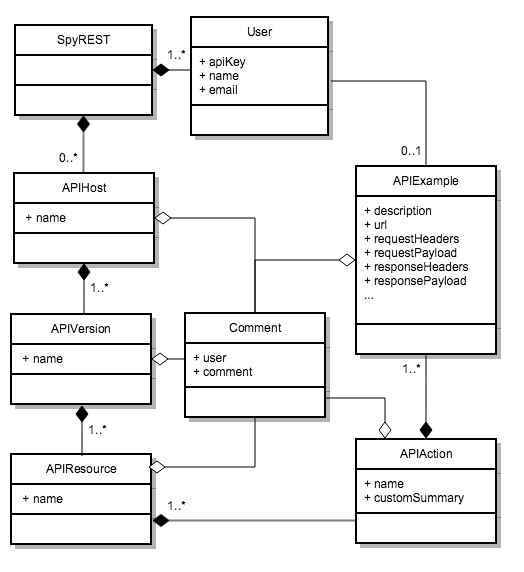
\includegraphics[width=\linewidth]{data_model.png}
  \caption{SpyREST data model}
  \label{fig:data_model}
\end{figure}

\begin{figure*}[!tbh]
  \centering
  \begin{subfigure}[t]{0.4\textwidth}
    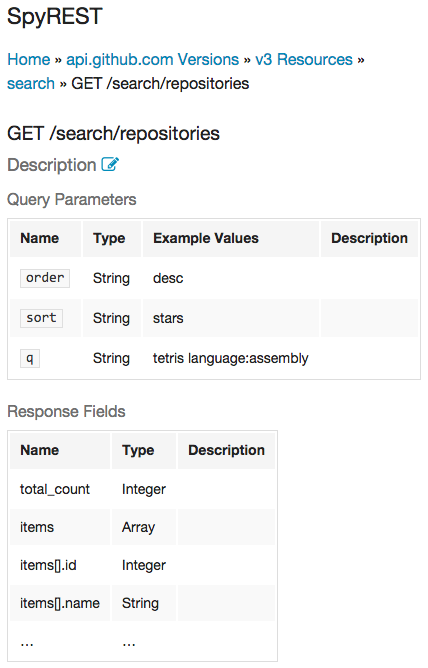
\includegraphics[width=\linewidth]{spyrest_header.png}
    \caption{API documentation summary section}
    \label{fig:summary}
  \end{subfigure}
  \begin{subfigure}[t]{0.5\textwidth}
    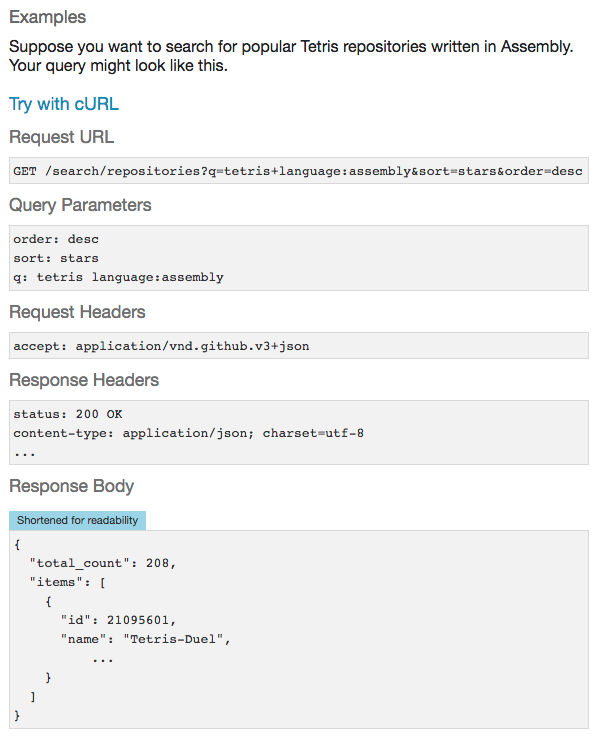
\includegraphics[width=\linewidth]{spyrest_examples.png}
    \caption{API documentation examples section}
    \label{fig:examples}
  \end{subfigure}
  \caption{Screenshots of the web app with auto generated API documentation}
  \label{fig:spyrest_screenshots}
\end{figure*}

To allow API developers to suppress the auto detection algorithms for version, resource and action fields, the proxy server can be provided with custom HTTP headers when example API calls are executed. For example, an API developer can use the custom header ``x-spy-rest-resource: repos'' when making example API calls to override the automatic detection of resource from ``repositories'' to ``repos''. Using a similar approach, API developers can override the version, action, and description fields using the ``x-spy-rest-version'', ``x-spy-rest-action'' and ``x-spy-rest-description'' headers respectively.

To allow the API developers run the example API calls multiple times, the Spy computes a digest to uniquely identify an API example. The digest is computed based on the version, resource, url and description fields that are extracted from the example. This allows API developers to auto update the documentation when an API changes using the existing examples without creating duplicates.

When saving request information, Spy automatically strips off values used in ``authorization'' request headers to avoid leaking secrets in the API documentation as recommended by Stepalina \cite{Stepalina_saas}. If an authorization header is found, Spy also marks the example with ``requiresAuth: true'' so that in the generated API documentation it can be visually indicated.

SpyREST allows users to sign up and get an API key to be used for generating API documentation. The ``apiToken'' and ``userId'' fields are populated when a valid SpyREST API key is provided in the ``x-spy-rest-api-key'' request header. This provides credibility to the documentation generated by SpyREST since the official API developers can be identified by their SpyREST account.

To record data for an example call to an API that uses a SSL/TLS connection, the Spy needs to perform as an intentional man-in-the-middle style proxy since the data would be encrypted otherwise. We consider the security risks for this approach to be minimal when the example API calls are intended to be recorded for public viewing through the documentation. For APIs where this is not acceptable, the Spy can be installed with the required SSL certificates on their trusted infrastructure to overcome this issue.

The Spy component is built using Node.js\footnote{https://nodejs.org/} and open source libraries and SpyREST currently supports JSON based APIs only.

\textbf{The Database:} The database component saves the data that is captured by the Spy and the web app. The Spy saves the recorded data about the API examples and the auto-computed meta data in the database. The web app saves data about SpyREST users and custom modifications on auto-generated API documentation on the same database. As shown in Fig. \ref{fig:data_model}, all the data models excluding the comments are saved in the database component. The comments are saved on Disqus\footnote{https://disqus.com}, a third-party service that features rich collaboration features for websites. Its document oriented feature allows the Spy to save arbitrary HTTP request and response data in the database. MongoDB\footnote{https://www.mongodb.org/}, a widely used document oriented database, is used to implement the database component. MongoDB's scalability features can be used by SpyREST to automatically generate documentation of large number of RESTful APIs in a shared platform.

\textbf{The Web App:} The web app component further processes and presents auto generated documentation that is captured by Spy in the database. The web app also allows the API developers to edit or add custom content to the auto generated documentation. Additionally, the web app includes administration features such as user registration and SpyREST API key management. The features of the web app are discussed later in this paper in greater detail. The web app is written using the Ruby on Rails\footnote{http://rubyonrails.org/} framework primarily because of the first author's past experience using this framework.

The source code for both the Spy and web app components are released as open source projects. The specific technologies used by SpyREST work as an example implementation of the core technique of using an HTTP proxy server to auto generate RESTful API documentation.

\subsection{SpyREST Features} % (fold)

Now that we have explained the three components of SpyREST and how they work, we discuss how SpyREST meets the aforementioned requirements R1-7.

\textbf{R1 - Automated RESTful API documentation:} The work flow for automated RESTful API documentation can be explained by the following steps: 1) API developer uses the Spy HTTP proxy to run example API calls, 2) The Spy records example API calls, 3) The Spy extracts meta information about the API call, 4) The Web app displays the auto generated documentation, 5) API developers can optionally customize the auto generated documentation.

Fig \ref{fig:spyrest_screenshots} shows some screen shots  (content and presentation adapted for brevity) of fragments from SpyREST auto generated documentation that is solely based on an example API call to URL \url{https://api.github.com/search/repositories?q=tetris+language:assembly&sort=stars&order=desc} with a custom header ``x-spy-rest-description'' to provide the short description for the example.

To show both the structure and the example usages of the API, the auto-generated API documentation features two sections, a summary section as shown in Fig. \ref{fig:summary} and an examples section as shown in Fig. \ref{fig:examples}. The summary section shows a breadcrumb containing the hierarchy of the API objects related to each API action to help API client developers easily navigate the API documentation as a tree. This section also includes three tables that display the structure of query parameters, and request and response payloads. In addition to the structure, automated type detection is used to show the data type for each field in these tables. Example values are also automatically populated for query parameters. This reduces the need for a manual effort by automating the process based on the recorded data.

The examples section on the API documentation shows all the recorded API examples for a given API action. For each example, it shows a description, the request URL, query parameters, and request and response headers and bodies. Because Spy filters out the ``authorization'' request header before saving the examples in the database, the documentation rendered by the web app displays this header with a placeholder text as ``FILTERED''. As discussed before, the Spy also computes a ``strippedResponseBody'' by truncating large arrays in API responses to contain only two samples per array. The web app displays this ``strippedResponseBody'' to limit the verbosity on the auto-generated API documentation. Not shown in Fig. \ref{fig:spyrest_screenshots} for brevity, each example in the documentation also shows the information about the API developer that ran the API example and the time when it was generated.

\textbf{R2 - Example based:} SpyREST generated RESTful API documentation includes both the structure of the API objects and concrete examples for different use cases. The API examples are annotated with user provided descriptions through the custom headers that are otherwise hard to automatically infer. Because the Spy computes a hash digest for uniquely identifying each API example, replays of the same API example only updates the auto-generated documentation with the latest information allowing API developers to update the API documentation automatically when the API changes during development time. To record the examples in SpyREST, any REST API client can be used as long as it supports an HTTP proxy to call the API.

\textbf{R3 -  Executable documentation:} SpyREST keeps a copy of the API request information including URL, headers and request body. As a result, SpyREST can also recreate the example API calls that can be executed by users of the generated API documentation. Currently, it automatically generates executable test cases that can be run using cURL\footnote{http://curl.haxx.se/}. cURL is a command line based tool that can be used as a REST API client. The examples section on Fig. \ref{fig:examples} shows a link titled ``Try with cURL'', on click of which the user gets a panel with an executable API call example reconstructed from the recorded data as shown in Fig. \ref{fig:curl}.

\begin{figure}[!tbh]
  \centering
  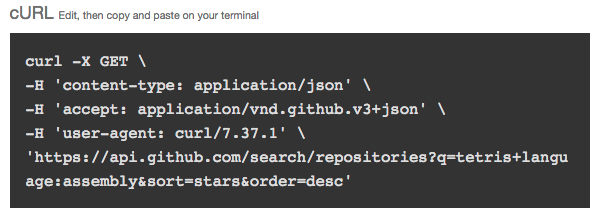
\includegraphics[width=\linewidth]{curl.png}
  \caption{Executable Examples in SpyREST using cURL}
  \label{fig:curl}
\end{figure}

This panel containing the executable API example is editable on the user interface. The editable panel allows the API client developers to modify the API call if they need to customize the auto-generated API call. For example, to change the value of ``order'' query parameter from ``desc'' to ``asc''  as shown in Fig. \ref{fig:curl}, a user can edit the text in this panel before executing the API example in cURL. Although not currently implemented, similar to cURL, SpyREST can generate executable tests targeting other REST API clients and programming languages since the required information to reconstruct an executable test is already available in the database.

\begin{table}[!tbh]
  \caption{Examples of auto detected versions}
  \begin{tabular}{|p{0.2\linewidth}|p{0.5\linewidth}|p{0.2\linewidth}|}
    \hline
    Type & Example Value & Detected version\\
    \hline
    ``accept'' header & application/vnd.ex.ca.v3+json & v3\\
    \hline
    ``accept'' header & application/vnd.ex.ca.v3.1+json & v3.1\\
    \hline
    URL & \url{/v2/x} & v2\\
    \hline
    URL & \url{/v2.1/x} & v2.1\\
    \hline
    URL & \url{/v2.1-pre/users} & v2.1-pre\\
    \hline
  \end{tabular}
  \label{table:versions}
\end{table}

\textbf{R4 - Version awareness:} SpyREST allows API developers to publish the documentation for multiple versions of their RESTful APIs. To organize API documentations and examples under multiple versions, SpyREST has an automatic version detection algorithm that parses the ``accept'' request header or the URL. Table \ref{table:versions} shows some examples of auto-detected versions. To cover the commonly used versioning schemes, the version detection logic tokenizes the ``accept'' header and URL to find segments that are prefixed with a ``v'' followed by numbers. In case this heuristic fails to detect a version, the examples are recorded under ``Default'' version. If required, the auto version detection algorithm can be suppressed by specifying the version in the custom ``x-spy-rest-version'' header when running example API calls through the Spy in.

\textbf{R5 - Customizable:} SpyREST allows API developers to modify and add custom free-form contents to the auto generated summary section of the documentation using Markdown\footnote{\url{http://en.wikipedia.org/wiki/Markdown}} syntax. Markdown was chosen because of its popularity as a documentation and code sharing tool among software developers on platforms such as StackOverflow and GitHub. SpyREST solely relies on example calls to APIs to auto-generate the API documentations. Custom content can be used to provide overview information and explain complicated business rules about the APIs that are not derivable from simply synthesizing the examples. We consider this as a pragmatic solution to augment manual effort with the largely automated solution to the RESTful API documentation effort. The summary section on the API documentation page has a button next to the ``Description'' title that opens up the Markdown editor with preview support as shown in Fig. \ref{fig:markdown}. As shown in this example, a user can annotate the auto-generated documentation for the ``order'' query parameter as being an ``optional field''. The custom edits are persisted in the database and are not overridden when the API examples are replayed unless the user decides to revert back to automated summaries.

\begin{figure}[!tbh]
  \centering
  \begin{subfigure}[t]{0.5\linewidth}
    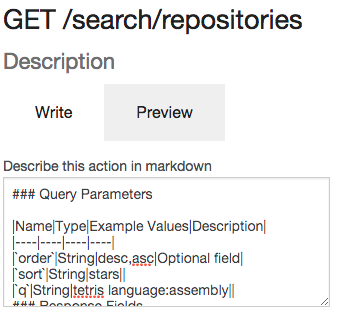
\includegraphics[width=\linewidth]{edit.png}
    \caption{Editing auto-generated summary}
  \end{subfigure}
  \begin{subfigure}[t]{0.45\linewidth}
    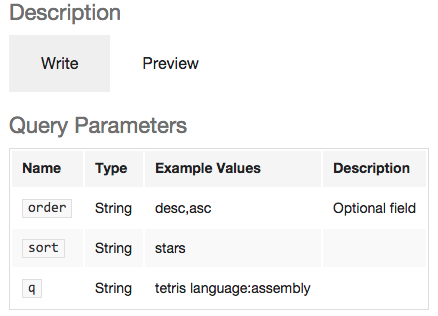
\includegraphics[width=\linewidth]{preview.png}
    \caption{Previewing customized content}
  \end{subfigure}
  \caption{Screen shots showing customization feature}
  \label{fig:markdown}
\end{figure}

\textbf{R6 - Reusable:} SpyREST only relies on an HTTP proxy to auto-generate RESTful API documentation. So, it can be used to document RESTful APIs that are developed using any underlying technology. To feed SpyREST with data, any REST API client can be used as long as it supports connecting through an HTTP proxy server. This technology agnostic feature allows SpyREST to be a reusable RESTful API documentation tool.

SpyREST is offered as a SaaS tool that can be used to auto-generate and publish documentation of multiple RESTful APIs. For APIs where a SaaS solution is not acceptable, SpyREST can also be installed and used as a self-hosted solution. Because SpyREST is an open-source application, users can modify the source to support any unique requirements that are not supported by SpyREST.

\begin{figure}[!tbh]
  \centering
  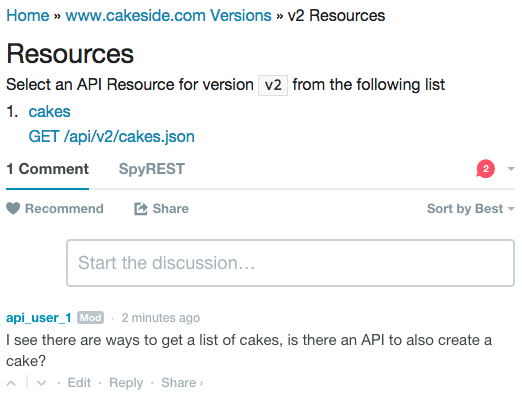
\includegraphics[width=\linewidth]{comments.png}
  \caption{SpyREST screen shot showing collaboration}
  \label{fig:comments}
\end{figure}


\textbf{R7 - Collaborative:} SpyREST allows the API developers to comment and discuss API related questions with API client developers right next to the documentation so that crowdsourced documentations can coexist with the officially published API documentation. The current implementation of commenting features on SpyREST is based on disqus\footnote{https://disqus.com/} as shown in the Fig. \ref{fig:comments}. Each API documentation page on SpyREST features its own discussion thread to help users easily locate relevant information.

\section{SpyREST Case-Study}
Now that we have discussed the different features offered by SpyREST, in this section we discuss a case study of using SpyREST to auto generate the documentation of one API action from the GitHub API. GitHub currently publishes a manually generated documentation of their API at: \url{https://developer.github.com/v3/}.

We start by looking at the manually written notifications list API available at \url{https://developer.github.com/v3/activity/notifications/#list-your-notifications}. Using this API, a GitHub user can fetch notifications about different activities related to their account. To auto-generate the documentation for this API using SpyREST, we need to make some example API calls via the Spy proxy. To make the example API calls, in this demonstration, we use a REST client using a Ruby program as follows:

\lstset{showstringspaces=false, basicstyle=\footnotesize, numbers=left, numbersep=1pt }
\begin{lstlisting}[language=ruby, breaklines=true, caption={}, label=list:ex]
class Github
  include HTTParty

  base_uri 'https://api.github.com'
  headers('Accept' => 'application/vnd.github.v3+json',
    'User-Agent' => 'curl/7.37.1',
    'content-type' => 'application/json',
    'Authorization' => "token GITHUB_API_TOKEN'"
  )

  host, port = 'spyrest.com', 9081
  http_proxy host, port
end

describe 'Notifications' do

  it 'List all notifications for the current user, where they are participating, since a time' do

    response = Github.get '/notifications?all=true&participating=true&since=2014-01-01T00:00:00Z'

    assert_equal 200, response.code
  end

end\end{lstlisting}

To auto-generate the API documentation for notifications API in GitHub, we first setup the base URL and required HTTP request headers on lines 4-6 inside the \texttt{Github} class. Next, we setup the proxy connection to go through the Spy on line 12. The \texttt{Github} class is defined once and used for all example API calls. Then we provide an example API call describing a use case for the \texttt{/notifications} action on lines 15-22 that use the \texttt{Github} class. Additional API examples can be provided using code similar to line 15-22. This example is written as an automated test using the RSpec testing framework\footnote{\url{http://rspec.info/}} so that in addition to generating the API documentation, API developers can use the same code as functional tests for the API and vice versa, essentially performing ``test driven documentation''. With this setup, when the tests are run, it executes the example API calls and SpyREST automatically generates the API documentation for the \texttt{/notifications} action.


\begin{figure}[!tbh]
  \centering
  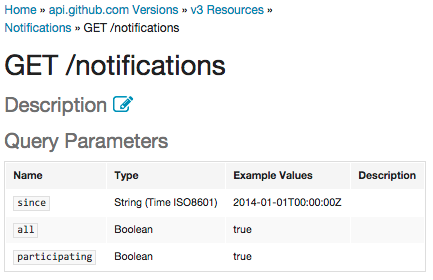
\includegraphics[width=\linewidth]{notifications_query.png}
  \caption{Screen shot showing URL query parameters}
  \label{fig:notifications_query}
\end{figure}

Fig. \ref{fig:notifications_query} shows a screen shot of the auto generated summary table for the URL query parameters associated with the \texttt{api.github.com > v3 > notifications > GET /notifications} API action. This table merges the different parameters such as \texttt{all, participating and since}, from the four example API calls to the \texttt{/notifications} API and displays the auto-detected data type such as ISO8601 formatted time, as well as example values that are captured. Similarly, SpyREST also automatically displays the structure of the API request and response bodies, if any, on separate tables using a similar visualization as shown in Fig. \ref{fig:spyrest_screenshots}. A user can edit this auto generated summary information using a Markdown editor in the UI to provide further details and customize the auto generated summary.

\begin{figure}[!tbh]
  \centering
  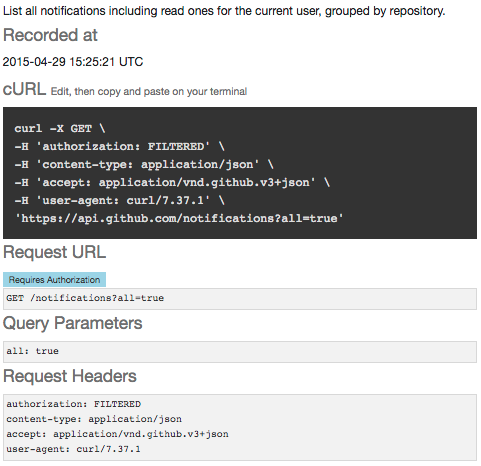
\includegraphics[width=\linewidth]{notification_example.png}
  \caption{Screen shot of documentation with an example use}
  \label{fig:notification_example}
\end{figure}

In addition to showing the structure of the API objects, SpyREST displays the actual data collected from the four example APIs on the auto generated documentation. Fig. \ref{fig:notification_example} shows a fragment of the documentation for the example API call generated from line 15 on the test code. On line 8 of our test code, we set the required \texttt{authorization} header for GitHub. The Spy does not save this secret value and the auto-generated documentation displays \texttt{authorization: FILTERED} in the Request Headers section as shown in Fig. \ref{fig:notification_example}. SpyREST also automatically includes a ``Requires Authorization'' message on the documentation because of the presence of this \texttt{authorization} header. SpyREST auto generates the cURL command to allow users to execute this example API call without writing any code. As discussed earlier, SpyREST features a commenting section on every API documentation page to allow API client developers to collaborate and find relevant information on the APIs.

In this case study, we have shown how a total of 24 lines of executable test code, including 7 blank lines, has been used to auto-generate the documentation of the \texttt{/notifications} action for the Github API. We consider the effort required for writing the test code to be simpler than the effort that'd be required to manually write an API documentation by looking at the content and presentation of the auto generated documentation. Moreover, when the API changes, a replay of the test code will automatically update the documentation. Using a similar approach, we have used SpyREST to auto generate documentation for 21 API actions randomly sampled from three RESTful API providers\footnote{\url{https://github.com/smsohan/spyrest_examples}}: GitHub.com, KISSMetrics.com, and CakeSide.com.

Even though Ruby and RSpec test framework have been used in this demonstration, any RESTful API client can be used instead. An automated way to run the example APIs are preferred since it is easier to repeat and maintain than a manual approach. We recommend using a test framework because it combines the benefits of both automated testing and documentation from the same effort.

\section{Discussion}
RESTful API documentation is expensive and error-prone because of the manual effort involved in the process. Our core contribution is a novel approach where an HTTP proxy server is used to largely automate the process for RESTful API documentation. There is a lack of tool support for automatically generating documentation of RESTful APIs. We presented SpyREST as an example implementation of the HTTP proxy server based solution to fill this need. SpyREST demonstrates how HTTP proxies can be used to automatically record and synthesize the recorded data from example API calls to provide a pragmatic solution for automatic RESTful API documentation. In the previous section, we demonstrated a case study showing how to use SpyREST to auto generate documentation for a GitHub API. Similar to this demonstration, RESTful APIs for different applications can be documented from executable code that are easier to maintain over a manual editing process.

The requirements for SpyREST are derived from analyzing the existing literature and industry practices as well as our own experiences developing RESTful APIs and their documentation. In the literature, several papers provided lists of recommendations for API documentation based on studying the existing tools and techniques and feedback collected from API developers. We found a lack of available tool support to generate RESTful API documentation following those recommendations and worked on SpyREST to provide a solution. As a result, SpyREST features such as automated documentation with executable examples, customizable contents, collaboration, version awareness and reusability provide a ready to use tool support for RESTful API documentation following the recommendations.

As demonstrated by SpyREST, the novel approach of using an HTTP proxy sever offers some unique benefits over existing tools from the academia and the industry. For example, tools that rely on user provided comments on source code and code inspection, such as JavaDoc, require the user to write formatted comments that are often applicable to a single programming language. The comments are not executable, and manual effort is required to ensure the comments and the API that it describes are kept in sync. The verbose nature of RESTful API documentation caused by the different parts such as URL parameters, headers, request and response body, and examples makes it difficult to write and maintain as comments in source code. Using an HTTP proxy server, SpyREST offers a language agnostic solution so that RESTful APIs written in any programming language can be documented using a single tool.

Another key feature of SpyREST is the shared platform for publishing RESTful API documentation so that API developers do not need to maintain a whole website on their own to publish their API documentation. A similar shared platform is provided by several other tools such as Swagger, Blueprint, etc. We identify the key advantage of SpyREST over these tools to be the fact that SpyREST relies on example API calls instead of relying on a custom API specification that are required by these tools. As discussed in section \ref{sec:related_work}, several authors have also published specifications for describing RESTful APIs. To generate these API specifications, a manual effort is required since there is no automated tools available to do so. The work flow for using these API specification formats can be described as follows: (1) execute example API calls $\longrightarrow$ (2) manually generate API specification $\longrightarrow$ (3) automatically generate API documentation. SpyREST does not rely on any custom API specification, so the associated manual effort can be largely avoided resulting in a smaller work flow as follows: (1) execute example API calls $\longrightarrow$ (2) automatically generate API documentation. We consider this as a significant cost saving approach for APIs with several endpoints or APIs that evolve.

When APIs are documented following a specification, the documentation produced is machine readable that can be used by API clients to automatically infer some business rules. Although not implemented in the current version, the data captured by SpyREST can be exported to partially auto generate the API documentation according to these specifications so that API developers can work on the remaining parts that need customization leaving the repeated parts to SpyREST. Another difference between the commercially available solutions such as Swagger, Blueprint, etc. is that SpyREST can be used both as a shared and a self-hosted platform. The self-hosted mode can be used for documenting internal RESTful APIs that cannot be released on the internet or customizing the open-sourced code of SpyREST to fit unique API specific needs.

While SpyREST offers an automated solution for documenting RESTful APIs, API developers can customize the auto generated content. Several authors in the literature identified the need for rich content comprising of text and diagrams to explain complex business rules about some APIs. To achieve this goal, we consider augmenting auto generated documentation with user contributed documentation, when necessary, to provide a pragmatic solution.

To summarize, from our example implementation of SpyREST and the case-study, we have found the proposed HTTP proxy server based solution offers several benefits over the existing techniques for RESTful API documentation.

\subsection{Threats to Validity} % (fold)
\label{sub:threats_to_validity}

\textbf{Internal Threats.} Our proposed technique uses an HTTP proxy server that can only intercept and record the data when it is either in clear text or trusted to be decrypted by SpyREST using an intentional man-in-the-middle approach. Because SpyREST can be used as a shared platform, any secrets used in the example API calls get decrypted in memory, even though not saved by SpyREST. To overcome these threat, we recommend API developers to use disposable secrets so that the secrets used to run an API call are valid for a single API call. For use cases where this is unacceptable, the self-hosted mode can be used as an alternative.

The current implementation of SpyREST is limited to work on JSON based RESTful APIs only. When generating the summary tables to show the structure for API actions with URL parameters, request and response bodies, SpyREST parses the JSON payloads associated with the example API calls. JSON based APIs are supported because of their widespread use among popular RESTful APIs such as Twitter, Facebook, Google Maps. To achieve similar documentation for APIs using other formats such as XML, CSV, etc., the same concepts are applicable, but would require additional implementation.

\textbf{External Threats.}  We have used SpyREST to auto generate documentation for APIs randomly sampled from three RESTful API providers as a proof of concept and found the proxy server based solution met the requirements R1-7. Further evaluation is needed in our future work involving RESTful API developers and users to understand and improve the effectiveness of the SpyREST features over a larger set of RESTful APIs.

\section{Conclusion}
In this paper, we have introduced a novel technique of using an HTTP proxy server to auto generate RESTful API documentation. With SpyREST, we have shown an implementation of the technique and compared its advantages over existing techniques related to RESTful API documentation. The proxy server based solution supports integrated features such as automated RESTful API documentation with executable example API calls, support for multiple versions, customization and collaboration that are offered both as a SaaS and self-hosted platforms. These features have been recommended by existing research on the documentation of APIs. We have demonstrated using SpyREST with automated test code so that RESTful API documentation can be achieved as a positive side-effect of executing automated tests. Overall, based on the outcome of our work on SpyREST, we conclude that a proxy server based approach shows a pragmatic solution to the RESTful API documentation problem.

In future, we will perform and report a qualitative user study involving developers and users of RESTful APIs to find out the strengths and shortcomings of SpyREST compared to the existing solutions. In addition to incorporating the feedback collected from the user study, we will continue our research on the evolution of RESTful APIs to extend the HTTP proxy server based technique to better support the documentation needs for RESTful APIs that evolve.

\bibliographystyle{IEEEtran}
\bibliography{IEEEabrv,references}


\end{document}


